\documentclass[12pt,]{article}
\usepackage{lmodern}
\usepackage{amssymb,amsmath}
\usepackage{ifxetex,ifluatex}
\usepackage{fixltx2e} % provides \textsubscript
\ifnum 0\ifxetex 1\fi\ifluatex 1\fi=0 % if pdftex
  \usepackage[T1]{fontenc}
  \usepackage[utf8]{inputenc}
\else % if luatex or xelatex
  \ifxetex
    \usepackage{mathspec}
  \else
    \usepackage{fontspec}
  \fi
  \defaultfontfeatures{Ligatures=TeX,Scale=MatchLowercase}
\fi
% use upquote if available, for straight quotes in verbatim environments
\IfFileExists{upquote.sty}{\usepackage{upquote}}{}
% use microtype if available
\IfFileExists{microtype.sty}{%
\usepackage{microtype}
\UseMicrotypeSet[protrusion]{basicmath} % disable protrusion for tt fonts
}{}
\usepackage[margin=1in]{geometry}
\usepackage{hyperref}
\hypersetup{unicode=true,
            pdftitle={Your Awesome Title},
            pdfauthor={Author One and Author Two},
            pdfborder={0 0 0},
            breaklinks=true}
\urlstyle{same}  % don't use monospace font for urls
\usepackage{longtable,booktabs}
\usepackage{graphicx,grffile}
\makeatletter
\def\maxwidth{\ifdim\Gin@nat@width>\linewidth\linewidth\else\Gin@nat@width\fi}
\def\maxheight{\ifdim\Gin@nat@height>\textheight\textheight\else\Gin@nat@height\fi}
\makeatother
% Scale images if necessary, so that they will not overflow the page
% margins by default, and it is still possible to overwrite the defaults
% using explicit options in \includegraphics[width, height, ...]{}
\setkeys{Gin}{width=\maxwidth,height=\maxheight,keepaspectratio}
\IfFileExists{parskip.sty}{%
\usepackage{parskip}
}{% else
\setlength{\parindent}{0pt}
\setlength{\parskip}{6pt plus 2pt minus 1pt}
}
\setlength{\emergencystretch}{3em}  % prevent overfull lines
\providecommand{\tightlist}{%
  \setlength{\itemsep}{0pt}\setlength{\parskip}{0pt}}
\setcounter{secnumdepth}{0}
% Redefines (sub)paragraphs to behave more like sections
\ifx\paragraph\undefined\else
\let\oldparagraph\paragraph
\renewcommand{\paragraph}[1]{\oldparagraph{#1}\mbox{}}
\fi
\ifx\subparagraph\undefined\else
\let\oldsubparagraph\subparagraph
\renewcommand{\subparagraph}[1]{\oldsubparagraph{#1}\mbox{}}
\fi

%%% Use protect on footnotes to avoid problems with footnotes in titles
\let\rmarkdownfootnote\footnote%
\def\footnote{\protect\rmarkdownfootnote}

%%% Change title format to be more compact
\usepackage{titling}

% Create subtitle command for use in maketitle
\newcommand{\subtitle}[1]{
  \posttitle{
    \begin{center}\large#1\end{center}
    }
}

\setlength{\droptitle}{-2em}
  \title{Your Awesome Title}
  \pretitle{\vspace{\droptitle}\centering\huge}
  \posttitle{\par}
  \author{Author One and Author Two}
  \preauthor{\centering\large\emph}
  \postauthor{\par}
  \predate{\centering\large\emph}
  \postdate{\par}
  \date{2017-04-26 11:44:43}

\usepackage{geometry}
\geometry{verbose,letterpaper,margin=2.45cm}

% \usepackage[breaklinks=true,pdfstartview=FitH,citecolor=blue]{hyperref}
\hypersetup{colorlinks,%
	citecolor=blue,%
	filecolor=red,%
	linkcolor=blue,%
	urlcolor=red,%
	pdfstartview=FitH}

\usepackage[T1]{fontenc}
\usepackage[utf8]{inputenc}
\usepackage{textgreek}
\usepackage[greek,english]{babel}
\usepackage{microtype}
\usepackage{amsmath}
\usepackage[osf]{libertine}
\usepackage{libertinust1math}
\usepackage{inconsolata}

\usepackage{booktabs}

\usepackage{setspace}
\doublespacing

% \setstretch{1.8999999999999999}

\usepackage{lineno}
\linenumbers

% \renewcommand{\rmdefault}{cmr}


% flush left while keep identation
\makeatletter
\newcommand\iraggedright{%
  \let\\\@centercr\@rightskip\@flushglue \rightskip\@rightskip
  \leftskip\z@skip}
\makeatother

\begin{document}
\maketitle

% align only at left, not at right.
\iraggedright

\textbf{Running headline}: Environment and species richness

\textbf{Abstract}: Your awesome abstract here.

\clearpage

\section{Introduction}\label{introduction}

Here is your introduction. It should describe clearly the rationale for
the study being done and the previous work related with the study. It
should also tell readers about your specific hypothese/questions being
addressed. Citations will be like this (Adair et al.
\protect\hyperlink{ref-adair_single-pool_2010}{2010}), or (e.g., Clark
and Tilman \protect\hyperlink{ref-clark_loss_2008}{2008}), or (Eriksson
and Ehrlén \protect\hyperlink{ref-eriksson_seed_1993}{1993}, Williamson
et al. \protect\hyperlink{ref-williamson_dissolved_1999}{1999})

Here is the second paragraph of the introduction.

\section{Methods}\label{methods}

Here is the method section. You can include equations easily. For inline
equations, use \(\text{var}(X) = p(1-p)\). For display equation, use

\[\text{var}(X) = p(1-p)\]

\subsection{Results}\label{results}

\paragraph{Tables}\label{tables}

Insert tables by \texttt{kable} in knitr package in R. Then
cross-reference it back with: see Table \ref{tab:tableName}.

\begin{table}

\caption{\label{tab:tableName}Caption here.}
\centering
\begin{tabular}[t]{rr}
\toprule
Plot & sprich\\
\midrule
3294 & 31\\
3297 & 28\\
3299 & 26\\
3330 & 27\\
\bottomrule
\end{tabular}
\end{table}

Put results inline, e.g.~the mean species richness is 28.

\paragraph{\texorpdfstring{Insert tables by \texttt{xtable} package in
R}{Insert tables by xtable package in R}}\label{insert-tables-by-xtable-package-in-r}

Show as Table. \ref{t:anova}:

\begin{table}[ht]
\centering
\caption{Caption here} 
\label{t:anova}
\begin{tabular}{lrrrrr}
  \toprule
 & Df & Sum Sq & Mean Sq & F value & Pr($>$F) \\ 
  \midrule
pH          & 1 & 4.58 & 4.58 & 4.77 & 0.2733 \\ 
  shade       & 1 & 8.45 & 8.45 & 8.80 & 0.2070 \\ 
  Residuals   & 1 & 0.96 & 0.96 &  &  \\ 
   \bottomrule
\end{tabular}
\end{table}

\paragraph{Insert tables by hand}\label{insert-tables-by-hand}

Show as Table. \ref{tab:byhand}:

\begin{longtable}[]{@{}llll@{}}
\caption{\label{tab:byhand} Caption here.}\tabularnewline
\toprule
Col A & Col B & Col C & Col D\tabularnewline
\midrule
\endfirsthead
\toprule
Col A & Col B & Col C & Col D\tabularnewline
\midrule
\endhead
row 1 & 190 & \(112 \pm 2\) & \(233 \pm 3\)\tabularnewline
\(\eta\) & 0.13 & 0.12 & 0.12\tabularnewline
\(\eta^2\) & 0.14 & 0.13 & 0.50\tabularnewline
\(\eta^3\) & 0.15 & 0.31 & 0.52\tabularnewline
\bottomrule
\end{longtable}

\paragraph{Figures}\label{figures}

Insert figure by code chunk. And cross-ref it back as Figure
\ref{fig:figName}.

\begin{figure}

{\centering \includegraphics{ms_files/figure-latex/figName-1} 

}

\caption{Your caption here.}\label{fig:figName}
\end{figure}

Or if you already have the figure: And cite it as Figure \ref{fig:fig2}.

\begin{figure}

{\centering 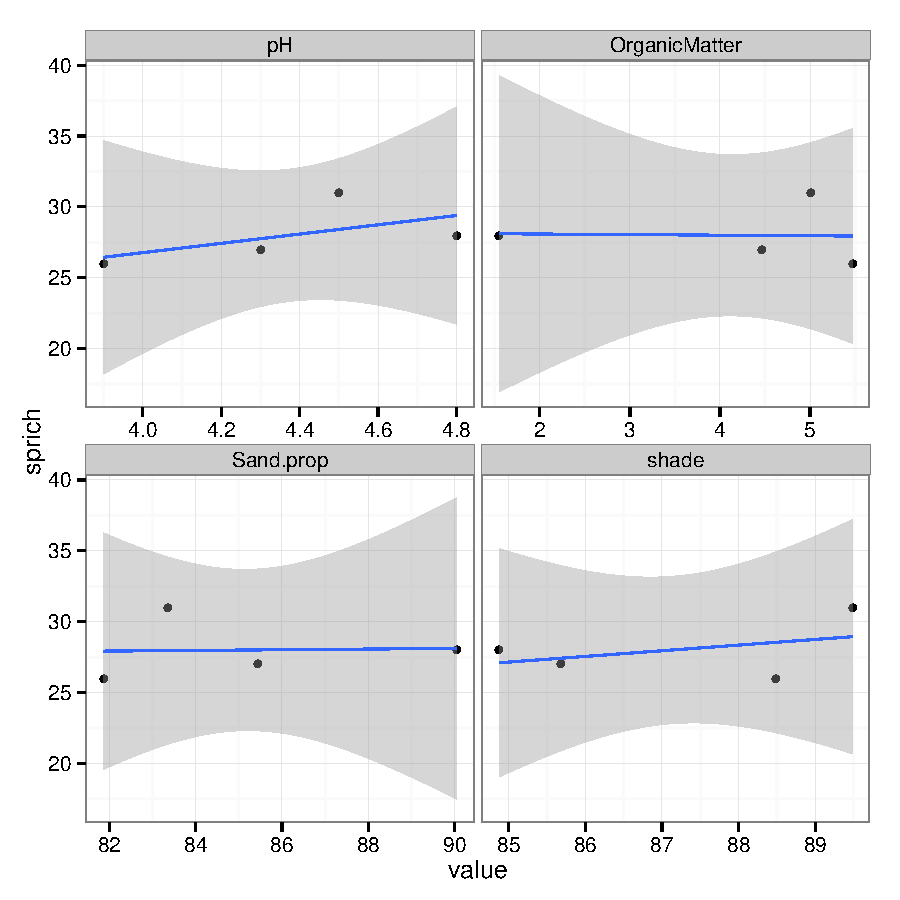
\includegraphics[width=0.7\linewidth]{/Users/dli/Github/workflow_demo/Figs/plot} 

}

\caption{Caption here.}\label{fig:fig2}
\end{figure}

More details can be found at
\href{https://bookdown.org/yihui/bookdown/}{here}.

\section*{References}\label{references}
\addcontentsline{toc}{section}{References}

\hypertarget{refs}{}
\hypertarget{ref-adair_single-pool_2010}{}
Adair, E. C. et al. 2010. Single-pool exponential decomposition models:
Potential pitfalls in their use in ecological studies. - Ecology 91:
1225--1236.

\hypertarget{ref-clark_loss_2008}{}
Clark, C. M. and Tilman, D. 2008. Loss of plant species after chronic
low-level nitrogen deposition to prairie grasslands. - Nature 451:
712--715.

\hypertarget{ref-eriksson_seed_1993}{}
Eriksson, O. and Ehrlén, J. 1993. Seed and microsite limitation of
recruitment in plant populations. - Oecologia 92: 361--366.

\hypertarget{ref-williamson_dissolved_1999}{}
Williamson, C. E. et al. 1999. Dissolved organic carbon and nutrients as
regulators of lake ecosystems: Resurrection of a more integrated
paradigm. - Limnology and Oceanography 44: 795--803.


\end{document}
